\includegraphics[height=1.25cm]{images/pictograms/aspect_logo}
\includegraphics[height=1.25cm]{images/pictograms/FEM}

%%%%%%%%%%%%%%%%%%%%%%%%%%%%%%%%%%%%%%%%%%%%%%%%%%%%%%%%%%%%%%%%%%%%%%%%%%%%%%%%%%%%%%%%%%%%%%%%%%%

\begin{flushright} {\tiny {\color{gray} python\_codes/fieldstone\_148/text.tex}} \end{flushright}

\lstinputlisting[language=bash,basicstyle=\small]{python_codes/fieldstone_148/keywords.key}

\par\noindent\rule{\textwidth}{0.4pt}

\begin{center}
\fbox{\textbf{\huge \color{teal} P}}
Code at \url{https://github.com/cedrict/fieldstone/tree/master/python_codes/fieldstone_148}
\end{center}

\par\noindent\rule{\textwidth}{0.4pt}

{\sl This stone was developed in collaboration with Erik van der Wiel}. \index{contributors}{E. van der Wiel}

\par\noindent\rule{\textwidth}{0.4pt}

%%%%%%%%%%%%%%%%%%%%%%%%%%%%%%%%%%%%%%%%%%%%%%%%%%%%%%%%%%%%%%%%%%%%%%%%%%%%%%%%%%%%%%%%%%%%%%%%%%%

%---------------------------------
\subsection*{Setup}

The domain is a 2D Cartesian box of size $L_x \times L_y$ which is discretised by means of 
$nelx \times nely$ elements. Both the $Q_2\times Q_1$ and $Q_2 \times P_{-1}$
element pairs are implemented, but given the discontinuous nature of the viscosity
field (see hereafter) the latter is to be preferred. 

Boundary conditions are free slip at the top and bottom while in/out-flow
kinematical boundary conditions are prescribed on the sides (see Section~\ref{abcd}). 
The in- to out-flow transition profile starts at a 150~\si{\km} depth and ends at a depth of 350~\si{\km}.
The prescribed velocities on the left and right lithosphere are $v_L$ and $v_R$ respectively.
Also an option ('symm bc') has been created so that the same outflow velocity is prescribed 
on the left and the right even though $|v_L| \neq |v_R$. Volume conservation is of course 
still ensured but it is in fact a case of absolute plate motion.
After solving the Stokes system, strain rate and deviatoric stress components are 
computed and projected onto nodes.

There are 6 materials in the domain (viscosity and density values are the default ones):
\begin{itemize}
\item Oceanic lithosphere ('o'):  
$\eta_o=10^{23}~\si{\pascal\second}$, $\rho_o=3300~\si{\kg\per\cubic\meter}$
\item Upper mantle ('um'): 
$\eta_{um}=10^{20}~\si{\pascal\second}$, $\rho_{um}=3500~\si{\kg\per\cubic\meter}$
\item Lower mantle ('lm'): 
$5\cdot 10^{22}~\si{\pascal\second}$, $ 3900~\si{\kg\per\cubic\meter}$ 
\item a D'' layer (dpp): 
$10^{21}~\si{\pascal\second}$,   $\rho_{dpp}=4000~\si{\kg\per\cubic\meter}$
\item two oceanic ridges coined A and B ('A', 'B'): 
$\eta_A=\eta_B=10^{19}$, $\rho_A=\rho_B=3300~\si{\kg\per\cubic\meter}$
\end{itemize}
For simplicity both viscosity and density are elemental fields, possibly discontinuous from 
one element to another.

Given the nature of the boundary conditions on all four sides 
the pressure can be computed up to a constant (nullspace)
so that we require that $\frac{1}{L_x}\int_{y=L_y} p dx =0$.
LINK to \textcite{joma22} (2022) - may be do it, as it would be 
much more consistent?

\begin{center}
\includegraphics[width=10cm]{python_codes/fieldstone_148/images/setup}
\end{center}


%---------------------------------
\subsection*{Experiments}

The code has been written in such a 
way that it can be scripted and the list of conducted experiments is presented in the following 
table. For reasons that need to be justified, experiment 4 has been deemed the reference one.


\begin{tabular}{lllllllll}
\hline
experiment & $v_L$ & $v_R$ & $\eta_{um}$ &rA &rB &o & $v_{mantle}$\\ 
\hline
\hline
1 & -4 &  4& 20&19&19&23&0\\
2 & -2 &  4& 20&19&19&23&0\\
3 & -4 &  8& 20&19&19&23&0\\
4 & -6 & 12& 20&19&19&23&0 & REF\\
5 & -8 & 16& 20&19&19&23&0\\
6 & -4 & 10& 20&19&19&23&0\\
7 & -8 &  8& 20&19&19&23&0\\
8 & -2 &  8& 20&19&19&23&0\\
9 & -4 & 15& 20&19&19&23&0\\
10& -4 & 20& 20&19&19&23&0\\
11& -6 & 12& 20       & {\bf 18} &  {\bf 18} & 23&0 & \\ 
12& -6 & 12& 20       & {\bf 20} &  {\bf 20} & 23&0 & \\ 
13& -6 & 12& {\bf 19} & 19       & 19        & 23&0\\
14& -6 & 12& {\bf 21} & 19       & 19        & 23&0\\
15& -6 & 12& 20       & 19       & 19        & {\bf 22}&0\\
16& -6 & 12& 20       & 19       & 19        & {\bf 24}&0\\
17& -6 & 12& 20       & 19       & 19        & {\bf 25}&0\\
18& -6 & 12& 20       & 19       & 19        & 23&0 & symm bc\\
19& -6 & 12& 20       & 19       & {\bf 18}  & 23&0&\\
20& -6 & 12& 20       & {\bf 18} & 19        & 23&0&\\
21& -6 & 12& 20       & {\bf 20} & 19        & 23&0&\\
22& -6 & 12& 20       &  19      & {\bf 20}  & 23&0&\\
23& -6 & 12& 20&19&19&23& {\bf 1} & \\
24& -6 & 12& 20&19&19&23& {\bf 3} & \\
25& -6 & 12& 20&19&19&23& {\bf 6} & \\
\hline
\end{tabular}

Additionally, mantle wind can be addedd ($v_{mantle}$). 

There are two simple ridges in the system, coined A and B. Each can have its own properties.
They are isosceles triangles. Ridge A is parameterised by points A,D,E while 
ridge B is parameterised by points B,F,H.

%---------------------------------
\subsection*{Measurements}
We focus on two profiles: $y=L_y$ and $x=L_x/2$ for which we export the velocity, 
the strain rate components, the pressure and the stress components.

Results are for now obtained with 300x150 but should ve rerun with 600x300 resolutions.

Todo/totry
\begin{itemize}
\item vary middle plate length
\item open bc + traction
\end{itemize}

\newpage

Horizontal profile at $y=Ly$:

\begin{center}
\includegraphics[width=8cm]{python_codes/fieldstone_148/results/fig1_exx_surface}
\includegraphics[width=8cm]{python_codes/fieldstone_148/results/fig1_u_surface}\\
\includegraphics[width=8cm]{python_codes/fieldstone_148/results/fig2_exx_surface}
\includegraphics[width=8cm]{python_codes/fieldstone_148/results/fig2_u_surface}\\
\includegraphics[width=8cm]{python_codes/fieldstone_148/results/fig3_exx_surface}
\includegraphics[width=8cm]{python_codes/fieldstone_148/results/fig3_u_surface}\\
\includegraphics[width=8cm]{python_codes/fieldstone_148/results/fig4_exx_surface}
\includegraphics[width=8cm]{python_codes/fieldstone_148/results/fig4_u_surface}\\
\includegraphics[width=8cm]{python_codes/fieldstone_148/results/fig5_exx_surface}
\includegraphics[width=8cm]{python_codes/fieldstone_148/results/fig5_u_surface}\\
\end{center}


\newpage

Vertical profile at $x=L_x/2$

\begin{center}
\includegraphics[width=8cm]{python_codes/fieldstone_148/results/fig1_exx_middle}
\includegraphics[width=8cm]{python_codes/fieldstone_148/results/fig1_u_middle}\\
\includegraphics[width=8cm]{python_codes/fieldstone_148/results/fig2_exx_middle}
\includegraphics[width=8cm]{python_codes/fieldstone_148/results/fig2_u_middle}\\
\includegraphics[width=8cm]{python_codes/fieldstone_148/results/fig3_exx_middle}
\includegraphics[width=8cm]{python_codes/fieldstone_148/results/fig3_u_middle}\\
\includegraphics[width=8cm]{python_codes/fieldstone_148/results/fig4_exx_middle}
\includegraphics[width=8cm]{python_codes/fieldstone_148/results/fig4_u_middle}\\
\includegraphics[width=8cm]{python_codes/fieldstone_148/results/fig5_exx_middle}
\includegraphics[width=8cm]{python_codes/fieldstone_148/results/fig5_u_middle}\\
\end{center}







%%%%%%%%%%%%%%%%%%%%%%%%%%%%%%%%%%%%%%%%%%%%%%%%%%%%%%%%%%%%%%%%%%%%%%%%%%%%%%%%%%%%%%%%%%%%%%%%%%%
\par\noindent\rule{\textwidth}{0.4pt}

\vspace{.5cm}

\begin{center}
\fbox{\begin{minipage}{0.9\textwidth}
{\color{teal}To Do, open questions, future work?}
\begin{itemize}
\item better lithostatic pressure ?
\item better open bc implementation
\end{itemize}
\end{minipage}}
\end{center}

%%%%%%%%%%%%%%%%%%%%%%%%%%%%%%%%%%%%%%%%%%%%%%%%%%%%%%%%%%%%%%%%%%%%%%%%%%%%%%%%%%%%%%%%%%%%%%%%%%%
\vspace{.5cm}

\Literature:\\
\fullcite{xxxxYY}


